\documentclass[tikz]{standalone}
\usetikzlibrary{shapes, calc, shapes, arrows, snakes}
\tikzset{dist/.style={path picture= {
    \begin{scope}[x=1pt,y=10pt]
      % \draw plot[domain=-6:6] (\x,{1/(1 + exp(-\x))-0.5});
      % \draw plot[domain=0:6] (\x,.5);
      % \draw plot[domain=-6:0] (\x,-.5);
      % \draw (0, -.5) -- (0, .5);
      \draw (-6, -.5) -- (0, -.5) -- (0, .5) -- (6, .5);
    \end{scope}
    }
  }
}
\tikzstyle{input}=[draw,fill=red!50,circle,minimum size=20pt,inner sep=0pt]
\tikzstyle{hidden}=[draw,fill=green!50,circle,minimum size=20pt,inner sep=0pt,dist]
\tikzstyle{output}=[draw,fill=white,circle,minimum size=20pt,inner sep=0pt]
\tikzstyle{bias}=[draw,dashed,fill=gray!50,circle,minimum size=20pt,inner sep=0pt]
\tikzstyle{layer}=[fill=gray!70]

\tikzstyle{stateTransition}=[->, thick]

\newcommand{\width}{0.2}
\begin{document}

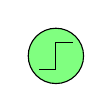
\begin{tikzpicture}[scale=2, >= stealth]
    % \fill[layer] (-\width,-1.7) rectangle (\width,1.7);
    % \fill[layer] (1+-\width,-1.7) rectangle (1+\width,1.7);
    % \fill[layer] (2+-\width,-1.7) rectangle (2+\width,1.7);
    % \fill[layer] (3+-\width,-1.7) rectangle (3+\width,1.7);
    % \node (l1label) at  (0, -1.9) {3};
    % \node (l2label) at  (1, -1.9) {64};
    % \node (l3label) at  (2, -1.9) {64};
    % \node (l4label) at  (3, -1.9) {1};
    % \node (r)[input,fill=red]   at (0, 1) {$s$};
    % \node (g)[input,fill=green] at (0, 0) {$s$};
    % \node (b)[input,fill=blue]  at (0,-1) {$s$};

    \node (h11)[hidden] at (1, 1.5) {};
    % \node (h12)[hidden] at (1, 0.5) {};
    % \node[circle,inner sep=0] (h13) at (1,-0.5) {\raisebox{5pt}{$\vdots$}};
    % \node (h14)[hidden] at (1,-1.5) {};
    % \node (h21)[hidden] at (2, 1.5) {};
    % \node (h22)[hidden] at (2, 0.5) {};
    % \node (h23) at (2,-0.5) {\vdots};
    % \node (h24)[hidden] at (2,-1.5) {};

    % \node (o1)[output] at (3,0) {$s$};

    % \draw[stateTransition] (r) -- (h11) node [midway,above=-0.06cm] {};
    % \draw[stateTransition] (r) -- (h12) node [midway,above=-0.06cm] {};
    % \draw[stateTransition] (r) -- (h13) node [midway,above=-0.06cm] {};
    % \draw[stateTransition] (r) -- (h14) node [midway,above=-0.06cm] {};
    % \draw[stateTransition] (g) -- (h11) node [midway,above=-0.06cm] {};
    % \draw[stateTransition] (g) -- (h12) node [midway,above=-0.06cm] {};
    % \draw[stateTransition] (g) -- (h13) node [midway,above=-0.06cm] {};
    % \draw[stateTransition] (g) -- (h14) node [midway,above=-0.06cm] {};
    % \draw[stateTransition] (b) -- (h11) node [midway,above=-0.06cm] {};
    % \draw[stateTransition] (b) -- (h12) node [midway,above=-0.06cm] {};
    % \draw[stateTransition] (b) -- (h13) node [midway,above=-0.06cm] {};
    % \draw[stateTransition] (b) -- (h11) node [midway,above=-0.06cm] {};

    % \draw[stateTransition] (h11) -- (h21) node [midway,above=-0.06cm] {};
    % \draw[stateTransition] (h11) -- (h22) node [midway,above=-0.06cm] {};
    % \draw[stateTransition] (h11) -- (h23) node [midway,above=-0.06cm] {};
    % \draw[stateTransition] (h11) -- (h24) node [midway,above=-0.06cm] {};
    % \draw[stateTransition] (h12) -- (h21) node [midway,above=-0.06cm] {};
    % \draw[stateTransition] (h12) -- (h22) node [midway,above=-0.06cm] {};
    % \draw[stateTransition] (h12) -- (h23) node [midway,above=-0.06cm] {};
    % \draw[stateTransition] (h12) -- (h24) node [midway,above=-0.06cm] {};
    % \draw[stateTransition] (h13) -- (h21) node [midway,above=-0.06cm] {};
    % \draw[stateTransition] (h13) -- (h22) node [midway,above=-0.06cm] {};
    % \draw[stateTransition] (h13) -- (h23) node [midway,above=-0.06cm] {};
    % \draw[stateTransition] (h13) -- (h24) node [midway,above=-0.06cm] {};
    % \draw[stateTransition] (h14) -- (h21) node [midway,above=-0.06cm] {};
    % \draw[stateTransition] (h14) -- (h22) node [midway,above=-0.06cm] {};
    % \draw[stateTransition] (h14) -- (h23) node [midway,above=-0.06cm] {};
    % \draw[stateTransition] (h14) -- (h21) node [midway,above=-0.06cm] {};

    % \draw[stateTransition] (h21) -- (o1) node [midway,above=-0.06cm] {};
    % \draw[stateTransition] (h22) -- (o1) node [midway,above=-0.10cm] {};
    % \draw[stateTransition] (h23) -- (o1) node [midway,above=-0.06cm] {};
    % \draw[stateTransition] (h24) -- (o1) node [midway,above=-0.06cm] {};

%     \draw [
%     thick,
%     decoration={
%         brace,
%         mirror,
%         raise=0.5cm
%     },
%     decorate
% ] (1+-\width, -1.8) -- (2+\width, -1.8)
% node [pos=0.5,anchor=north,yshift=-0.55cm] {50\% dropout};
\end{tikzpicture}
\end{document} 